\documentclass[11pt,a4paper]{article}
\usepackage[margin=2.2cm]{geometry}
\usepackage[T1]{fontenc}
\usepackage[utf8]{inputenc}
\usepackage{lmodern}
\usepackage{microtype}
\usepackage{amsmath,amssymb}
\usepackage{booktabs}
\usepackage{array}
\usepackage{enumitem}
\usepackage{caption}
\usepackage{subcaption}
\usepackage{graphicx}
\usepackage{xcolor}
\usepackage{tikz}
\usetikzlibrary{arrows.meta,positioning,calc,fit,backgrounds}
\usepackage{pgfplots}
\pgfplotsset{compat=1.17}
\usepackage[hidelinks]{hyperref}

\definecolor{cours}{HTML}{3B6EA8}
\definecolor{coccam}{HTML}{3D9A6B}
\definecolor{cgrey}{HTML}{777777}
\definecolor{cwarn}{HTML}{B5532A}
\newcommand{\hit}{\textcolor{coccam}{$\bullet$}}
\newcommand{\miss}{\textcolor{cgrey}{$\circ$}}
\newcommand{\code}[1]{\texttt{\small #1}}
\makeatletter\newcommand{\inputtable}[1]{\@@input #1 }\makeatother

\title{\textbf{The Occam's LGS full chain}\\[2pt]
\large LangSplat SAM ViT-H features, Occam's lift, our query --- run, measurements, and comparison with our previous results}
\author{Radiance FYP --- semantic embedding\\ \small intellisense08 (RTX 2080, 8\,GB). Run 13--14 October 2026; report 16 October 2026}
\date{}

\begin{document}
\maketitle

\begin{abstract}
\noindent This document describes, step by step, the run of Occam's LGS as its authors use it, on our two scenes. The
2D language features come from LangSplat's preprocessing: SAM ViT-H masks at three granularities and one OpenCLIP
ViT-B/16 embedding per mask. These are lifted onto our trained Gaussians with Occam's centre-pixel estimator, one table
column group per granularity, and queried by our unchanged 3D query and evaluator. We compare it with our previous
results: our default lift (A teachers, multi-scale CLIP crops), the scale-averaged lift (Old), our SAM variant B2, and
the 13 October run of \emph{the same Occam's lift on our A teachers}. That last comparison isolates the 2D features. The
full chain finds \textbf{25 of 29} objects with \textbf{1 of 6} absent objects firing, against 22/29 with 2--3/6 for every
previous configuration. Holding the lift fixed, LangSplat's features account for +3 objects and $-2$ false positives. The
cost is one-off: 5.4\,h (backroom) and 4.7\,h (flightroom) of SAM extraction on the RTX 2080, then 30\,s to lift.
\end{abstract}

\tableofcontents
\clearpage

% ─────────────────────────────────────────────────────────────────────────────
\section{Summary}
\begin{center}\small
\resizebox{\linewidth}{!}{%
\begin{tabular}{lccccc}
\toprule
Configuration (Phase 5 sets, floor 0.55) & hits /29 & absent firing /6 & best hits at 1 FP & AUROC br / fr & median err (m)\\
\midrule
Ours, Old teachers & 20 & 2 & 19 & 0.85 / 0.90 & 0.19 / 0.22\\
Ours, A teachers (default since 8 Oct) & 22 & 2 & 19 & 0.87 / 0.90 & 0.21 / 0.25\\
Occam's lift on A teachers (13 Oct run) & 22 & 3 & --- & 0.87 / 0.92 & 0.26 / 0.18\\
\textbf{Occam's full chain (this run)} & \textbf{25} & \textbf{1} & \textbf{25} & \textbf{0.92 / 1.00} & 0.27 / 0.30\\
\bottomrule
\end{tabular}}
\end{center}
\begin{enumerate}[leftmargin=*,itemsep=2pt]
  \item \textbf{Best result measured on our scenes.} Backroom 12/13, flightroom 13/16, development set 5/5.
  \item \textbf{The features are the cause.} The same Occam's lift on our A teachers gave 22/29 and 3/6 false positives.
        Replacing only the 2D features with LangSplat's gives 25/29 and 1/6. On 13 Oct, replacing only the lift changed
        nothing.
  \item \textbf{Gains:} \emph{swivel chair}, \emph{camera tripod}, \emph{hose reel} (backroom) relative to A, with no
        losses. \emph{Office chair}, which Occam's lift on A missed, is found again. Flightroom's absent \emph{recycling bin}
        no longer fires.
  \item \textbf{Robust to the floor:} 25/29 with one false positive at every floor from 0.52 to 0.55; 24/29 at 0.575.
  \item \textbf{Costs:} localisation error +0.05\,m (median), and about 5 GPU-hours of feature extraction per scene.
  \item \textbf{Still missed by everything:} white bucket, keyboard, floor lamp, drone gate.
\end{enumerate}

% ─────────────────────────────────────────────────────────────────────────────
\section{The chain, step by step}

\begin{figure}[h]
\centering
\resizebox{\linewidth}{!}{%
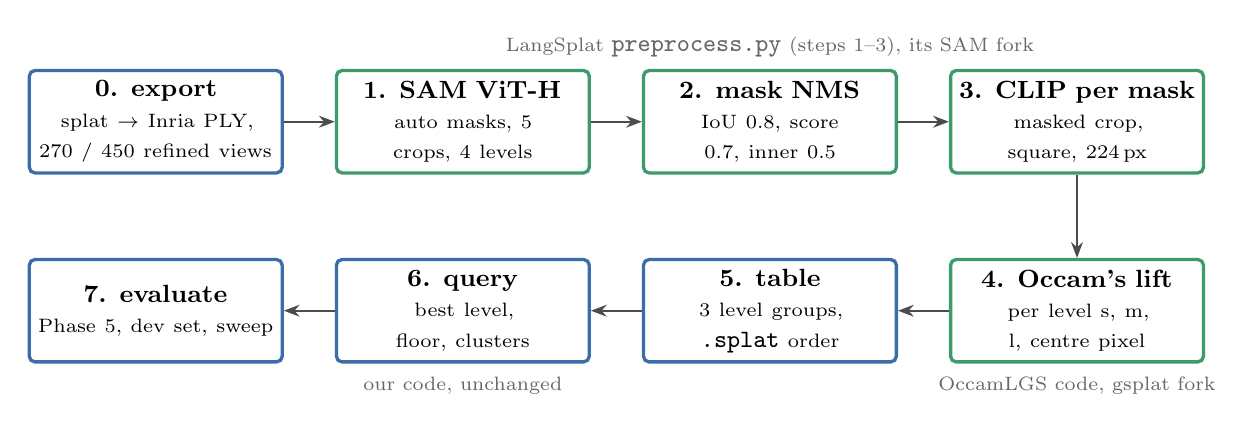
\begin{tikzpicture}[font=\small,
  box/.style={draw, rounded corners=2pt, align=center, minimum height=13mm, text width=30mm, inner sep=3pt, fill=white},
  occ/.style={box, draw=coccam, very thick}, ours/.style={box, draw=cours, very thick},
  arr/.style={-{Stealth[length=2mm]}, thick, draw=black!70}]
  \node[ours] (s0) at (0,0)    {\textbf{0. export}\\\scriptsize splat $\to$ Inria PLY, 270 / 450 refined views};
  \node[occ]  (s1) at (3.9,0)  {\textbf{1. SAM ViT-H}\\\scriptsize auto masks, 5 crops, 4 levels};
  \node[occ]  (s2) at (7.8,0)  {\textbf{2. mask NMS}\\\scriptsize IoU 0.8, score 0.7, inner 0.5};
  \node[occ]  (s3) at (11.7,0) {\textbf{3. CLIP per mask}\\\scriptsize masked crop, square, 224\,px};
  \node[occ]  (s4) at (11.7,-2.4) {\textbf{4. Occam's lift}\\\scriptsize per level s, m, l, centre pixel};
  \node[ours] (s5) at (7.8,-2.4) {\textbf{5. table}\\\scriptsize 3 level groups, \code{.splat} order};
  \node[ours] (s6) at (3.9,-2.4) {\textbf{6. query}\\\scriptsize best level, floor, clusters};
  \node[ours] (s7) at (0,-2.4) {\textbf{7. evaluate}\\\scriptsize Phase 5, dev set, sweep};
  \draw[arr] (s0) -- (s1); \draw[arr] (s1) -- (s2); \draw[arr] (s2) -- (s3); \draw[arr] (s3) -- (s4);
  \draw[arr] (s4) -- (s5); \draw[arr] (s5) -- (s6); \draw[arr] (s6) -- (s7);
  \node[font=\scriptsize, text=black!60] at (7.8,0.95) {LangSplat \code{preprocess.py} (steps 1--3), its SAM fork};
  \node[font=\scriptsize, text=black!60] at (11.7,-3.35) {OccamLGS code, gsplat fork};
  \node[font=\scriptsize, text=black!60] at (3.9,-3.35) {our code, unchanged};
\end{tikzpicture}}
\caption{The full chain. Green: the authors' code (LangSplat preprocessing, Occam's lift). Blue: our export, table
format, query and evaluator, unchanged from the earlier experiments.}
\label{fig:chain}
\end{figure}

\subsection*{Step 0 --- Export (\code{export\_scene.py}, kitchen env)}
The trained splatfacto Gaussians (backroom 532,361, flightroom 379,684) are written in the Inria PLY layout in checkpoint
order. The training views are written with the poses splatfacto refined (SO3$\times$R3 camera optimiser), the same 270 and
450 views our own lift uses. The images are linked unchanged.

\subsection*{Steps 1--3 --- LangSplat's language features (\code{langsplat\_features.py}, \code{occamlgs} env)}
Occam's paper lifts the feature maps LangSplat's \code{preprocess.py} produces. The runner imports that script's functions
and calls them with LangSplat's settings:
\begin{center}\small
\begin{tabular}{l>{\raggedright\arraybackslash}p{0.68\linewidth}}
\toprule
Image size & height $>1080$ is rescaled to 1080 (LangSplat's rule): backroom 1920$\times$1080, flightroom 1280$\times$720\\
SAM & ViT-H (\code{sam\_vit\_h\_4b8939}), LangSplat's fork of \code{segment-anything}\\
Automatic generator & 32 points per side, crop layers 1 (full image + 4 crops), predicted-IoU 0.7, box-NMS 0.7, stability 0.85, min region 100\,px\\
Granularities & the fork returns SAM's masks as \emph{default}, \emph{s} (subpart), \emph{m} (part), \emph{l} (whole)\\
Mask NMS & per level: score = stability $\times$ predicted IoU; IoU $>0.8$, score $<0.7$, inner-overlap 0.5 removed\\
CLIP input & mask's bounding box, pixels outside the mask set to black, padded square, resized to 224\,px\\
CLIP & OpenCLIP ViT-B/16 \code{laion2b\_s34b\_b88k} (the same model as our teachers), unit-norm, fp16\\
Output per image & \code{<stem>\_s.npy}: seg maps [4, H, W] (mask ids, $-1$ = none); \code{<stem>\_f.npy}: features [masks, 512]\\
\bottomrule
\end{tabular}
\end{center}

\begin{figure}[h]
\centering
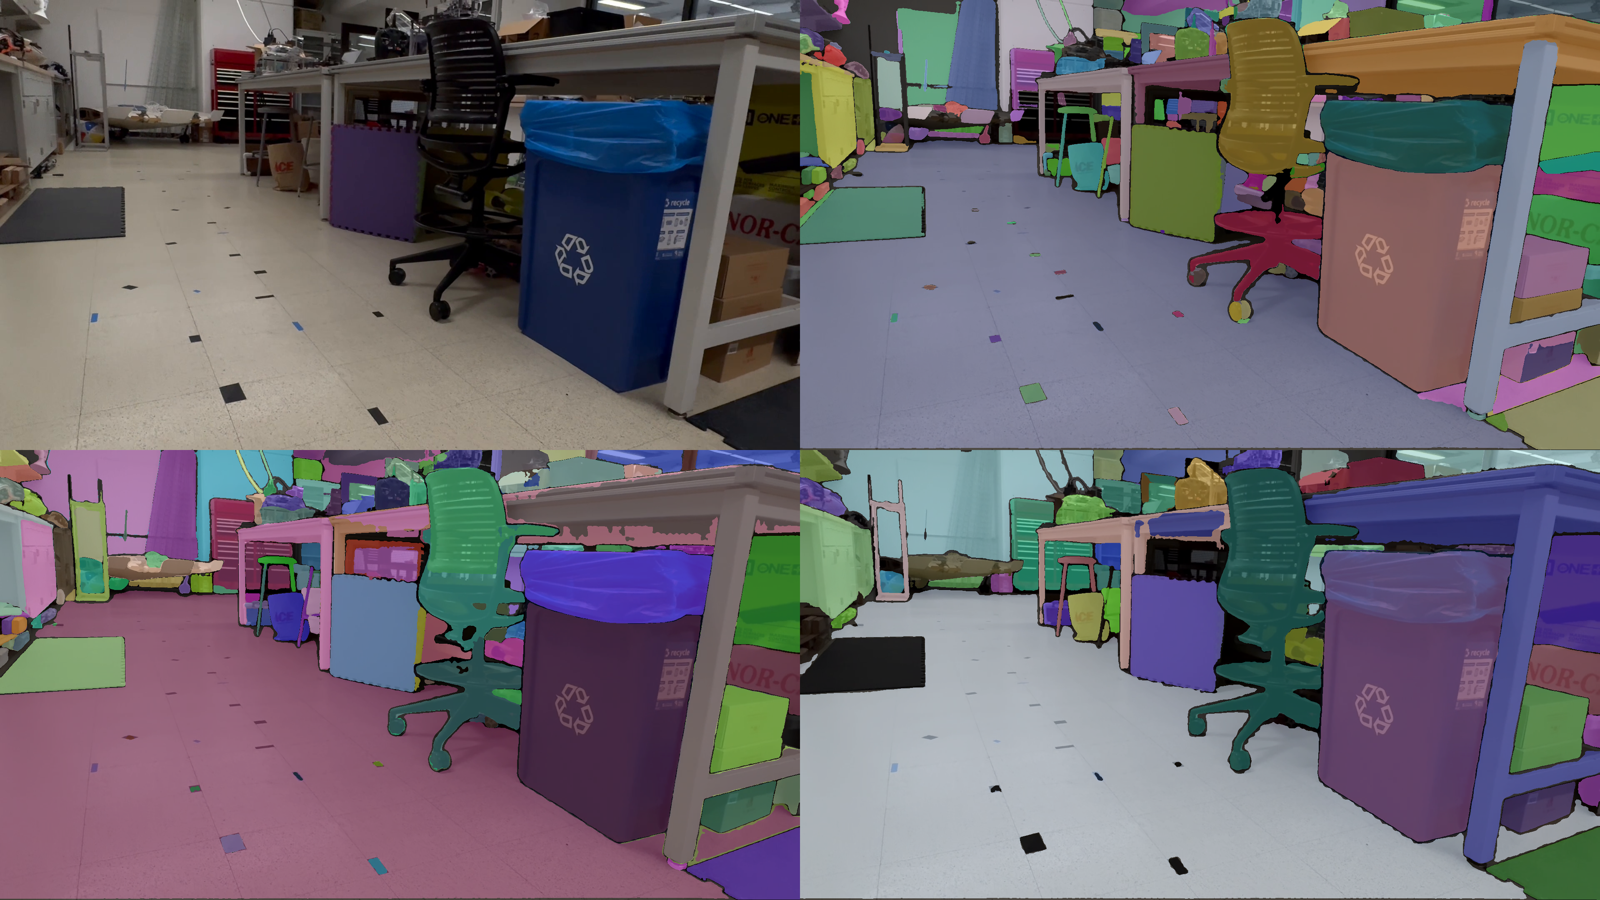
\includegraphics[width=0.49\linewidth]{../fig_levels_backroom.png}\hfill
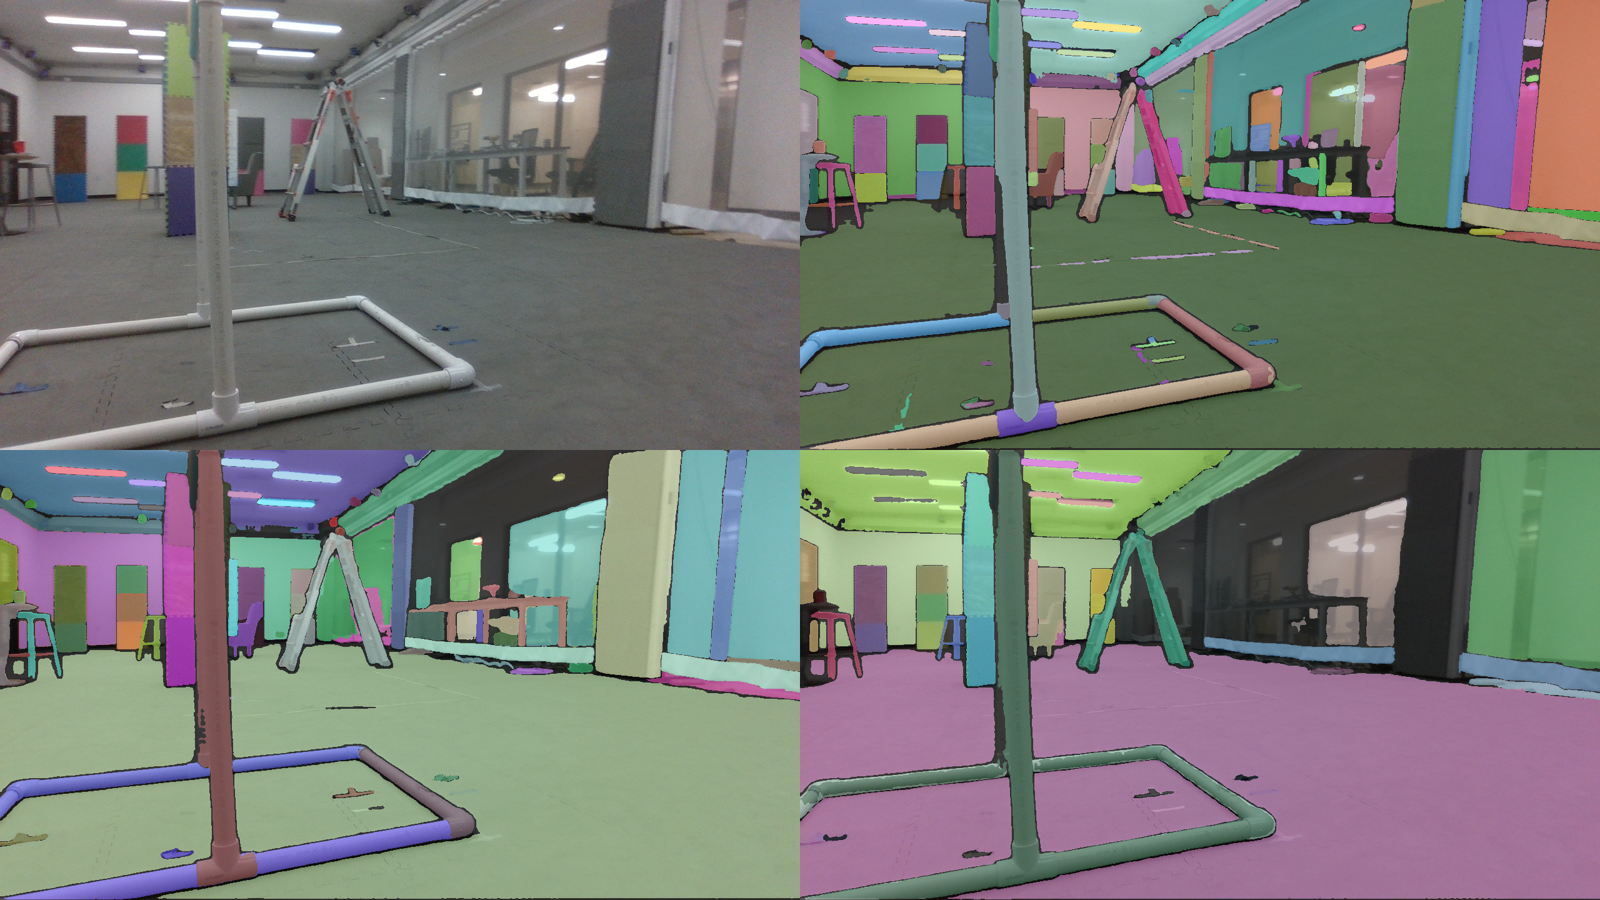
\includegraphics[width=0.49\linewidth]{../fig_levels_flightroom.png}
\caption{LangSplat's three granularities on one training image per scene (left: backroom frame 141; right: flightroom
frame 249). In each panel: top-left the image, top-right level s (subparts), bottom-left m (parts), bottom-right l (whole
objects). Each colour is one mask, i.e.\ one CLIP embedding. Uncovered pixels are dark. The chairs, the bin and the
benches are single segments at level l. These whole-object embeddings are what recover the occluded chairs.}
\label{fig:levels}
\end{figure}

\subsection*{Step 4 --- Occam's lift (\code{occam\_lift.py --langsplat}, \code{occamlgs} env)}
For each level $\ell\in\{s,m,l\}$ separately, Occam's renderer (gsplat fork) renders every training view at the seg-map
resolution. For every Gaussian $i$ blended at the pixel under its projected centre $\lfloor x_i'^v\rfloor$, it records
that blend weight $w_i^v$. Occam's \code{accumulate\_gaussian\_feature\_per\_view} then adds the feature of the mask covering
that pixel:
\begin{equation*}
f_i^{(\ell)}=\frac{\sum_v w_i^v\,m_\ell^v\,F_\ell^v\!\left(\lfloor x_i'^v\rfloor\right)}{\sum_v w_i^v\,m_\ell^v},\qquad
m_\ell^v=\mathbb 1\!\left[\text{a level-}\ell\text{ mask covers }\lfloor x_i'^v\rfloor\right].
\end{equation*}
Pixels that no mask covers do not contribute; this is Occam's \code{get\_language\_feature} mask. Gaussians never blended at
their own centre pixel get no feature. Occam's code prunes them; we keep them as zero rows with weight 0, so table rows
stay aligned with the \code{.splat} file. Seen: backroom 93.7\,\%, flightroom 91.8\,\% (our all-pixel lift: 99.9 / 99.6\,\%).

\subsection*{Step 5 --- Table (our \code{export} step, kitchen env)}
The three levels are stored as the table's three scale groups (\code{clip\_scales}), rows unit-normalised, in
\code{.splat} order (\code{lift\_occamfull}, 2.0\,GB backroom, 1.5\,GB flightroom). The mean of the three is stored as the
flat \code{clip} row.

\subsection*{Step 6 --- Query (our \code{run\_query}, unchanged)}
For a phrase, LERF relevancy (canonical phrases object / things / stuff / texture, temperature 10) is computed for each
level. The level whose top-100 relevancy is highest is used. That is LangSplat's own evaluation rule ("choose the level
with the highest relevancy"), and the same rule our A teachers use for crop scales. Then: floor 0.55, relative threshold
$\tau=0.55+0.5(\text{peak}-0.55)$, 0.1\,m voxel clusters of at least 15 Gaussians, top cluster, approach point at 1\,m.

\subsection*{Step 7 --- Evaluation}
The Phase 5 sets frozen on 6 Oct (backroom amended 7 Oct): 13 + 16 positives, 3 + 3 absent objects. A query hits if the
top cluster lies within 0.75\,m of an annotated instance or inside its padded box. The relevancy-floor sweep (0.46--0.60)
and the 5-query development set complete it. Nothing was tuned on these sets.

% ─────────────────────────────────────────────────────────────────────────────
\section{Running it on the RTX 2080}
\subsection{Problems met and how they were solved}
LangSplat and Occam's LGS were developed on 48\,GB GPUs. Three issues came up on the 8\,GB card. Each fix changes only
memory use or speed, not the numbers:
\begin{enumerate}[leftmargin=*,itemsep=2pt]
  \item \textbf{SAM decoder out of memory} on the second image: 64 prompt points per batch at 1080p. SAM decodes every
        point independently and merges batches before filtering, so \code{points\_per\_batch} 16 gives the same masks.
  \item \textbf{Mask NMS out of memory, then infeasible.} After 18 backroom images, one image produced 647 masks at one
        level. LangSplat's NMS compares every pair of full-resolution masks in a Python loop (5\,GB as a GPU copy; days
        per image on the CPU at that count). It is replaced by a vectorised version: a pairwise-intersection matrix of
        integer pixel counts, summed over pixel chunks on the GPU, with LangSplat's IoU and inner-overlap rules applied
        elementwise in the same order. Checked against LangSplat's own function on real masks (table below): identical
        selection on all 10 level sets, 10--40$\times$ faster.
  \item \textbf{Feature maps in memory.} A per-pixel 512-d map at 1080p is 4.2\,GB in fp32. It is held in fp16, the
        precision LangSplat stores the features in.
\end{enumerate}
The run then resumed from image 19, skipping the finished files. LangSplat's \code{create()} hides the real exception
behind \code{ValueError(1)}; that message in the first log is the NMS out-of-memory error.

\begin{center}\small
\resizebox{\linewidth}{!}{%
\begin{tabular}{lrrrr}
\toprule
Backroom training view, level & masks & kept (ours) & kept (LangSplat) & time ours / LangSplat (s)\\
\midrule
view 1, default / s / m / l & 180 / 143 / 89 / 27 & 58 / 109 / 46 / 22 & identical & 0.5 / 7.6\\
view 2, default / s / m / l & 305 / 240 / 160 / 60 & 101 / 168 / 98 / 39 & identical & 0.9 / 21.9\\
view 19, m / l & 336 / 142 & 209 / 101 & identical & 0.4 / 16.2\\
view 19, default / s & 647 / 496 & 247 / 319 & (loop not run) & 1.5\\
\bottomrule
\end{tabular}}
\end{center}

\subsection{Time and memory}
\begin{table}[h]
\centering\small
\caption{Extraction and lift. Per-image times are wall time of LangSplat's steps (SAM, NMS, CLIP); the sum includes the
first 18 backroom images from the first attempt. Peak GPU memory 5.9\,GB.}
\label{tab:timing}
\begin{tabular}{lcccccccc}
\toprule
Scene & image size & images & median s/img & p90 s/img & total (h) & lift (s) & seen (\%)\\
\midrule
\inputtable{tables/timing.tex}
\bottomrule
\end{tabular}
\end{table}

\begin{figure}[h]
\centering
\begin{tikzpicture}
\begin{axis}[ybar, width=0.9\linewidth, height=4.6cm, bar width=4pt, xlabel={seconds per image}, ylabel={images},
  legend style={font=\scriptsize, at={(0.98,0.95)}, anchor=north east}, grid=major, grid style={gray!20}, xmin=27, xmax=118]
  \addplot[fill=cours!60, draw=cours] table[x=lo, y=backroom, col sep=comma] {data/timing_hist.csv};
  \addplot[fill=coccam!60, draw=coccam] table[x=lo, y=flightroom, col sep=comma] {data/timing_hist.csv};
  \legend{backroom (1080p), flightroom (720p)}
\end{axis}
\end{tikzpicture}
\caption{LangSplat extraction time per image. SAM's automatic generator (5 crops $\times$ 1,024 prompts) dominates.}
\end{figure}

% ─────────────────────────────────────────────────────────────────────────────
\section{What the features look like}
\begin{table}[h]
\centering\small
\caption{Masks kept per image after NMS, per level (median and 10--90th percentile), and the share of pixels covered by
some mask (median, minimum over images). Levels s, m, l are lifted; \emph{default} is computed by LangSplat but not
used by Occam's lift.}
\label{tab:masks}
\begin{tabular}{llccccc}
\toprule
Scene & level & lifted & masks (median) & masks (p10--p90) & covered (\%) & min covered (\%)\\
\midrule
\inputtable{tables/masks.tex}
\bottomrule
\end{tabular}
\end{table}

\noindent Level s splits objects into parts (median 213 masks per backroom image), and l keeps whole objects (56). Each
level leaves 5--12\\,\\% of the pixels uncovered (floor, walls), and those pixels add nothing to any Gaussian. Our A and
Old teachers instead give every pixel a crop embedding, background included. In the table, 91--94\,\% of rows have a
feature at each level.

% ─────────────────────────────────────────────────────────────────────────────
\section{Comparison with our previous results}
\subsection{Headline}
\begin{table}[h]
\centering\small
\caption{Phase 5 evaluation, query settings unchanged since Phase 1. Per scene: hits, median and 90th-percentile
localisation error (m), absent objects returning a candidate, AUROC of peak relevancy (positives vs absent).}
\label{tab:headline}
\setlength{\tabcolsep}{3.2pt}
\resizebox{\linewidth}{!}{%
\begin{tabular}{lcc ccccc ccccc}
\toprule
& & & \multicolumn{5}{c}{backroom (13 + 3)} & \multicolumn{5}{c}{flightroom (16 + 3)}\\
\cmidrule(lr){4-8}\cmidrule(lr){9-13}
Configuration & hits & FP & hits & err & p90 & FP & AUROC & hits & err & p90 & FP & AUROC\\
\midrule
\inputtable{tables/headline.tex}
\bottomrule
\end{tabular}}
\end{table}

\paragraph{Same lift, different features.} "Occam lift, A" is the 13 Oct run: Occam's own lift code on our A
teachers (multi-scale CLIP crops, three scale groups). "Occam full" is the same lift on LangSplat's features (three SAM
levels). The only difference between the two rows is the 2D features, and it is worth +3 hits (22 $\to$ 25), $-2$ absent
objects firing (3 $\to$ 1), and higher AUROC on both scenes (0.87 $\to$ 0.92, 0.92 $\to$ 1.00).

\subsection{Per query}
\begin{table}[p]
\centering\small
\caption{Per positive query: hit (\hit) or miss (\miss) and peak relevancy for four configurations; for the full chain
also the chosen SAM level, the error to the nearest instance (m) and the failure kind. Bold queries differ between
configurations.}
\label{tab:perquery}
\setlength{\tabcolsep}{4pt}
\begin{tabular}{l cccc ccl}
\toprule
& Occam full & Occam lift, A & Ours A & Ours Old & level & err & failure (full)\\
\inputtable{tables/per_query.tex}
\bottomrule
\end{tabular}
\end{table}

\begin{itemize}[leftmargin=*,itemsep=2pt]
  \item \textbf{Occluded and thin objects gain most.} Flightroom's armchair (0.58 $\to$ 0.71 against A) and upholstered
        chair (0.55 $\to$ 0.65) sit behind the whiteboard in most views. A crop of fixed size around them contains mostly
        whiteboard; a SAM mask contains only the chair. The camera tripod (thin legs) rises from 0.54 to 0.59, just enough
        to clear the floor and form a cluster.
  \item \textbf{Swivel chair and office chair are both found} at level l. Our A table found the office chair but not the
        swivel chair; Occam's lift on A found neither.
  \item \textbf{Hose reel}, mounted on the ceiling and lost when A replaced Old, is found again at level l, and the camera tripod at level m.
  \item \textbf{Remaining misses.} White bucket: wrong object 1.8\,m away. Keyboard: peak 0.556, just over the floor
        but no cluster of 15 Gaussians. Floor lamp and drone gate: the right area, but the cluster centroid 0.87 and
        0.97\,m off. No configuration in either experiment has found these four.
  \item \textbf{Some peaks fall} (flightroom red cup 0.75 $\to$ 0.67, poster 0.74 $\to$ 0.67) without losing the hit. A
        mask-level embedding of a small object is less distinctive than a tight crop at the right scale, but still enough.
\end{itemize}

\begin{figure}[h]
\centering
\begin{tikzpicture}
\begin{axis}[width=0.62\linewidth, height=6.2cm, xlabel={peak relevancy, Ours A}, ylabel={peak relevancy, Occam full},
  xmin=0.36, xmax=0.86, ymin=0.36, ymax=0.86, grid=major, grid style={gray!20},
  legend style={font=\scriptsize, at={(0.02,0.98)}, anchor=north west}]
  \addplot[only marks, mark=*, coccam, mark size=1.8pt] table[x=a, y=occam, col sep=comma] {data/peaks_pos.csv};
  \addplot[only marks, mark=x, cwarn, mark size=3pt, thick] table[x=a, y=occam, col sep=comma] {data/peaks_neg.csv};
  \addplot[black!50, dashed, domain=0.36:0.86] {x};
  \addplot[black!40, dotted, thick] coordinates {(0.36,0.55) (0.86,0.55)};
  \addplot[black!40, dotted, thick] coordinates {(0.55,0.36) (0.55,0.86)};
  \legend{objects in the scene, absent objects, $y=x$, floor 0.55}
\end{axis}
\end{tikzpicture}
\caption{Peak relevancy per query, our A lift against the full chain (both scenes). Points above the diagonal rose. The
absent objects (crosses) moved down or stayed; flightroom's recycling bin crossed below the floor.}
\label{fig:peaks}
\end{figure}

\subsection{Absent objects}
\begin{table}[h]
\centering\small
\caption{Absent objects: whether a candidate is returned (fires) and the peak relevancy.}
\label{tab:absent}
\begin{tabular}{lcccc}
\toprule
Absent object & Occam full & Occam lift, A & Ours A & Ours Old\\
\midrule
\inputtable{tables/absent.tex}
\bottomrule
\end{tabular}
\end{table}

\noindent Only backroom's \emph{ceiling fan} still fires (peak 0.65). It fires in every configuration and at every floor,
which makes a real look-alike in the room likely (HANDOVER \S2.5); it should be verified in the photos.

\subsection{Which level the query chooses}
\begin{table}[h]
\centering\small
\caption{Level or scale group chosen per positive query (counts). SAM levels s / m / l for the full chain; crop-scale
groups small / medium / large for the A teachers.}
\label{tab:levels}
\begin{tabular}{l ccc ccc}
\toprule
& \multicolumn{3}{c}{backroom (13)} & \multicolumn{3}{c}{flightroom (16)}\\
\cmidrule(lr){2-4}\cmidrule(lr){5-7}
Configuration & s / S & m / M & l / L & s / S & m / M & l / L\\
\midrule
\inputtable{tables/levels.tex}
\bottomrule
\end{tabular}
\end{table}

\begin{table}[h]
\centering\small
\caption{Full chain: per level, median peak over the positive queries and highest peak over the absent objects.}
\label{tab:levelpeaks}
\begin{tabular}{l cc cc cc}
\toprule
& \multicolumn{2}{c}{level s} & \multicolumn{2}{c}{level m} & \multicolumn{2}{c}{level l}\\
\cmidrule(lr){2-3}\cmidrule(lr){4-5}\cmidrule(lr){6-7}
Scene & pos.\ median & absent max & pos.\ median & absent max & pos.\ median & absent max\\
\midrule
\inputtable{tables/level_peaks.tex}
\bottomrule
\end{tabular}
\end{table}

\noindent The query never picks the subpart level for an object in the scene, as A never picks its small-crop group.
Whole objects (l) are chosen for 22 of 29 queries. Level l also separates best: on flightroom its median positive peak
(0.66) is 0.13 above the highest absent peak, against 0.06 at level s. Choosing among the three adds two hits over
averaging them (the flat variant: 23/29 at one false positive, \S\ref{sec:sweep}).

\subsection{Relevancy-floor sweep}\label{sec:sweep}
\begin{figure}[h]
\centering
\begin{subfigure}{0.49\linewidth}
\begin{tikzpicture}
\begin{axis}[width=\linewidth, height=5.4cm, xlabel={relevancy floor}, ylabel={top-1 hits (of 29)}, ymin=14, ymax=27,
  legend style={font=\tiny, at={(0.5,-0.3)}, anchor=north, legend columns=2}, grid=major, grid style={gray!20}]
  \addplot[cours, thick, mark=*, mark size=1.2pt] table[x=floor, y=Old_hits, col sep=comma] {data/sweep.csv};
  \addplot[cours, thick, dashed, mark=square*, mark size=1.2pt] table[x=floor, y=A_hits, col sep=comma] {data/sweep.csv};
  \addplot[coccam, very thick, mark=diamond*, mark size=1.6pt] table[x=floor, y=Occamfull_hits, col sep=comma] {data/sweep.csv};
  \addplot[coccam, thick, dashed, mark=o, mark size=1.4pt] table[x=floor, y=Occamfullflat_hits, col sep=comma] {data/sweep.csv};
  \legend{Ours Old, Ours A, Occam full, Occam full (no level choice)}
\end{axis}
\end{tikzpicture}
\caption{Hits vs floor.}
\end{subfigure}\hfill
\begin{subfigure}{0.49\linewidth}
\begin{tikzpicture}
\begin{axis}[width=\linewidth, height=5.4cm, xlabel={absent objects with a candidate (of 6)}, ylabel={top-1 hits (of 29)},
  ymin=14, ymax=27, xmin=-0.5, xmax=6.5, legend style={font=\tiny, at={(0.5,-0.3)}, anchor=north, legend columns=2},
  grid=major, grid style={gray!20}]
  \addplot[cours, only marks, mark=*] table[x=Old_fp, y=Old_hits, col sep=comma] {data/sweep.csv};
  \addplot[cours, only marks, mark=square] table[x=A_fp, y=A_hits, col sep=comma] {data/sweep.csv};
  \addplot[coccam, only marks, mark=diamond*, mark size=3pt] table[x=Occamfull_fp, y=Occamfull_hits, col sep=comma] {data/sweep.csv};
  \addplot[coccam, only marks, mark=o, mark size=2.5pt] table[x=Occamfullflat_fp, y=Occamfullflat_hits, col sep=comma] {data/sweep.csv};
  \legend{Ours Old, Ours A, Occam full, Occam full (no level choice)}
\end{axis}
\end{tikzpicture}
\caption{Hits vs false positives (one point per floor).}
\end{subfigure}
\caption{Floors 0.46--0.60, both scenes combined. Old and A from the 13 Oct sweep.}
\end{figure}

\noindent At one false positive the full chain finds 25/29, against 19/29 for Old and A. At five false positives (floor
0.46) Old and A reach 24/29 and the full chain stays at 25. It stays at 24--25 from floor 0.46 to 0.575, while Old's
and A's trade hits for false positives throughout. These floors are read off the evaluation set, which is optimistic for
every curve alike.

% ─────────────────────────────────────────────────────────────────────────────
\section{Assessment}
\paragraph{What changed and why it helps.} The previous designs embed square crops of fixed sizes: a 7-scale pyramid
averaged (Old) or kept in three groups (A). Such a crop mixes the object with whatever surrounds it. LangSplat embeds each
SAM mask alone, on black, at the scale of the object. The CLIP embedding therefore describes the object rather than a
neighbourhood. That matters most when the object is occluded (the chairs behind the whiteboard) or thin (the tripod),
exactly where the crop designs failed. It also explains the better rejection of absent objects: a segment-level
embedding of a bin-shaped object in flightroom is less "recycling bin"-like than a crop containing bin-like context.

\paragraph{Caveats.} The improvement is three queries on 29 (3 gains, 0 losses against A; exact sign test $p=0.25$).
It is supported by fewer false positives, higher AUROC and a flat floor curve, but a larger, independently annotated
query set is still needed. The annotations were placed by Claude from photos, independently of all methods. Median
localisation error is 0.05\,m higher, because whole-object segments spread relevancy over the object's far side.
\emph{default}-level masks are computed but unused, as in Occam's code.

\paragraph{Relation to our B2.} B2 (8 Oct) also used SAM regions: ViT-B, levels by mask area, pyramid features where no
mask covers a pixel. It reached 21/29. Four differences remain untested one by one: ViT-H with a crop layer, SAM's own
granularities, skipping uncovered pixels instead of filling them, and LangSplat's mask NMS. With the LangSplat masks now
cached, each can be checked by re-lifting (30\,s) instead of re-extracting (hours).

\paragraph{Recommendation.} Make region-level features the base of \code{semantic/new}: SAM masks at three
granularities, one CLIP embedding per masked crop, a training-free lift per level, and the level chosen per query. Next
steps, in order:
\begin{enumerate}[leftmargin=*,itemsep=1pt]
  \item Ablate skip vs fill on the cached masks.
  \item Reduce extraction cost: no crop layer, fewer prompts, SAM~2 or an efficient SAM, on the RTX 5060 Ti.
  \item Anchor the goal on the object's visible surface to recover the 0.05\,m.
  \item Address the four objects no design finds, with a stronger recogniser or a re-ranker on the top candidates.
\end{enumerate}

% ─────────────────────────────────────────────────────────────────────────────
\section{Reproduction and files}
{\scriptsize
\begin{verbatim}
# branch semantic/LGS, repo root
source semantics/baselines/env.sh occamlgs
python semantics/baselines/langsplat_features.py --scene backroom          # 5.4 h on the RTX 2080 (resumable)
python semantics/baselines/occam_lift.py --scene backroom \
       --langsplat ~/Radiance/third_party/langsplat_features --suffix _occamfull
source ~/Radiance/figs/figs_env.sh
python figs/semantic_pipeline.py --scene backroom --backend lift --table-suffix _occamfull \
       --clip-mode scales --only export
cd semantics && python -m radiance_semantics.evaluate --scene backroom --variants L-C@occamfull
\end{verbatim}
}
\begin{itemize}[leftmargin=*,itemsep=1pt]
  \item Raw results: \code{../../raw/eval/} (Phase 5), \code{raw/eval\_dev/}, \code{raw/occam/} (levels chosen, masks per
        image, timing, table coverage), \code{raw/logs/} (run logs and the NMS check).
  \item Scripts: \code{../../scripts/occam\_analysis.py} (kitchen, CPU) and \code{make\_occam\_tables.py} regenerate every
        table and plot here.
  \item Host: the LangSplat cache (15\,GB) at \code{\textasciitilde/Radiance/third\_party/langsplat\_features/}; tables
        \code{lift\_occamfull} under each scene's \code{semantics/<run>/}.
  \item The joint report on both papers' full pipelines (with LUDVIG): \code{../full\_pipelines\_report.pdf}.
\end{itemize}

\end{document}
